\documentclass[11pt, logo, nonumbering]{preprint}
\usepackage[utf8]{inputenc}
\usepackage{microtype}
\usepackage{graphicx}
%\usepackage{times}
\usepackage{amsmath}
\usepackage{booktabs}
\usepackage{xcolor}
\definecolor{mydarkblue}{rgb}{0,0.08,0.45}
\usepackage[colorlinks=true,linkcolor=mydarkblue,citecolor=mydarkblue,filecolor=mydarkblue,urlcolor=mydarkblue]{hyperref}
\usepackage{xspace}
\usepackage{cleveref}

\usepackage[style=numeric-comp,maxbibnames=3,minnames=1,backend=bibtex, doi=false,eprint=false,url=false]{biblatex}
% \setlength{\bibsep}{0pt}

\addbibresource{ref.bib}

% Custom colors for your paper
\definecolor{gred}{RGB}{250, 210, 207}
\definecolor{coolblue1}{rgb}{0.91, 0.94, 0.98}
\definecolor{coolblue2}{rgb}{0.76, 0.85, 0.94}
\definecolor{coolblue3}{rgb}{0.54, 0.72, 0.87}
\definecolor{coolblue4}{rgb}{1, 1, 1}

% Custom commands for your paper
\newcommand{\ourbench}{\textsc{YourBenchmark}\xspace}
\newcommand{\ourbenchmini}{\texttt{YourBenchmark-mini}\xspace}
\newcommand{\ourbenchnum}{XXX\xspace}
\newcommand{\ourmodel}{YourModel\xspace}
\newcommand{\ourbaseline}{YourBaseline\xspace}






% for tableofcontent
% \usepackage{tocloft}
% \renewcommand{\contentsname}{\hfill\bfseries\Large Contents\hfill}   
% \renewcommand{\cftaftertoctitle}{\hfill}
% \renewcommand{\listtablename}{\hfill\bfseries\Large List of Tables} % no \hfill after "List of Tables"...
%%% using the command "\renewcommand{\cftlottitlefont}{\hfill\bfseries\Large}" works too...
% \renewcommand{\cftafterlottitle}{\hfill}


% Custom styling (add your own as needed)


\newcommand{\method}{LingoLLM\xspace}


\begin{document}

\title{\method: Your Paper Title Here} 
 

\author{
\textbf{Author Name}$^{1}$ \quad
\textbf{Another Author}$^{1}$ \quad
\textbf{Third Author}$^{1}$ \\
\textsuperscript{1}Carnegie Mellon University, Language Technologies Institute\\
\texttt{\{author1, author2, author3\}@cs.cmu.edu} \\
    \href{https://github.com/your-username/your-repo}{
\includegraphics[height=0.4cm]{logo/github.png} \textbf{your-username/your-repo}} ~ ~ ~ \href{https://huggingface.co/datasets/your-username/your-dataset}{
\includegraphics[height=0.4cm]{logo/huggingface.png} \textbf{your-username/your-dataset}}
    % Alternative without logos (comment above and uncomment below to use):
    % \href{https://github.com/your-username/your-repo}{\textbf{GitHub: your-username/your-repo}} ~ ~ ~ \href{https://huggingface.co/datasets/your-username/your-dataset}{\textbf{HF: your-username/your-dataset}} 
}

\maketitle


\begin{abstract}
The first sentence: what is the important problem in this paper. 
Second sentence: existing methods have limitations or challenge to solve the problem. 
Third sentence: In this paper, we propose \method, a novel method to xxxx. 
Fourth sentence: key insight or intuitive or novelty of the method. 
Fifth sentence: We evaluate \method on xxx public datasets, compared with xxx baselines. 
Experiments show that our proposed \method outperforms prior best methods by xxxx points ..... 

\end{abstract}

\section{Introduction}
\label{sec:intro}



Paragraph 1: overview of the larger problem domain, why it is important

Paragraph 2: Challenges of tackling the problem. what is the limitations of the prior methods. 

Paragraph 3: We propose xxxx. the key intuition and insights of the proposed method. 


The contributions of this paper are as follows:
\begin{itemize}[nosep]
    \item We propose \method, xxxx.
    %\item We use the successive decoding strategy to achieve the joint modeling of ASR and ST tasks.
    \item We xxxx
    \item \method outperforms prior best methods by xxx points. It achieves the state-of-the-art results on two popular benchmark datasets. 
\end{itemize}
We will make the model and code public available.

\section{Related Work}
\label{sec:related}
Put related work into categories. and discussion relation with the proposed work. \cite{example2023}

\section{Proposed Method}
\label{sec:method}


\begin{figure}[htb]
    \centering
    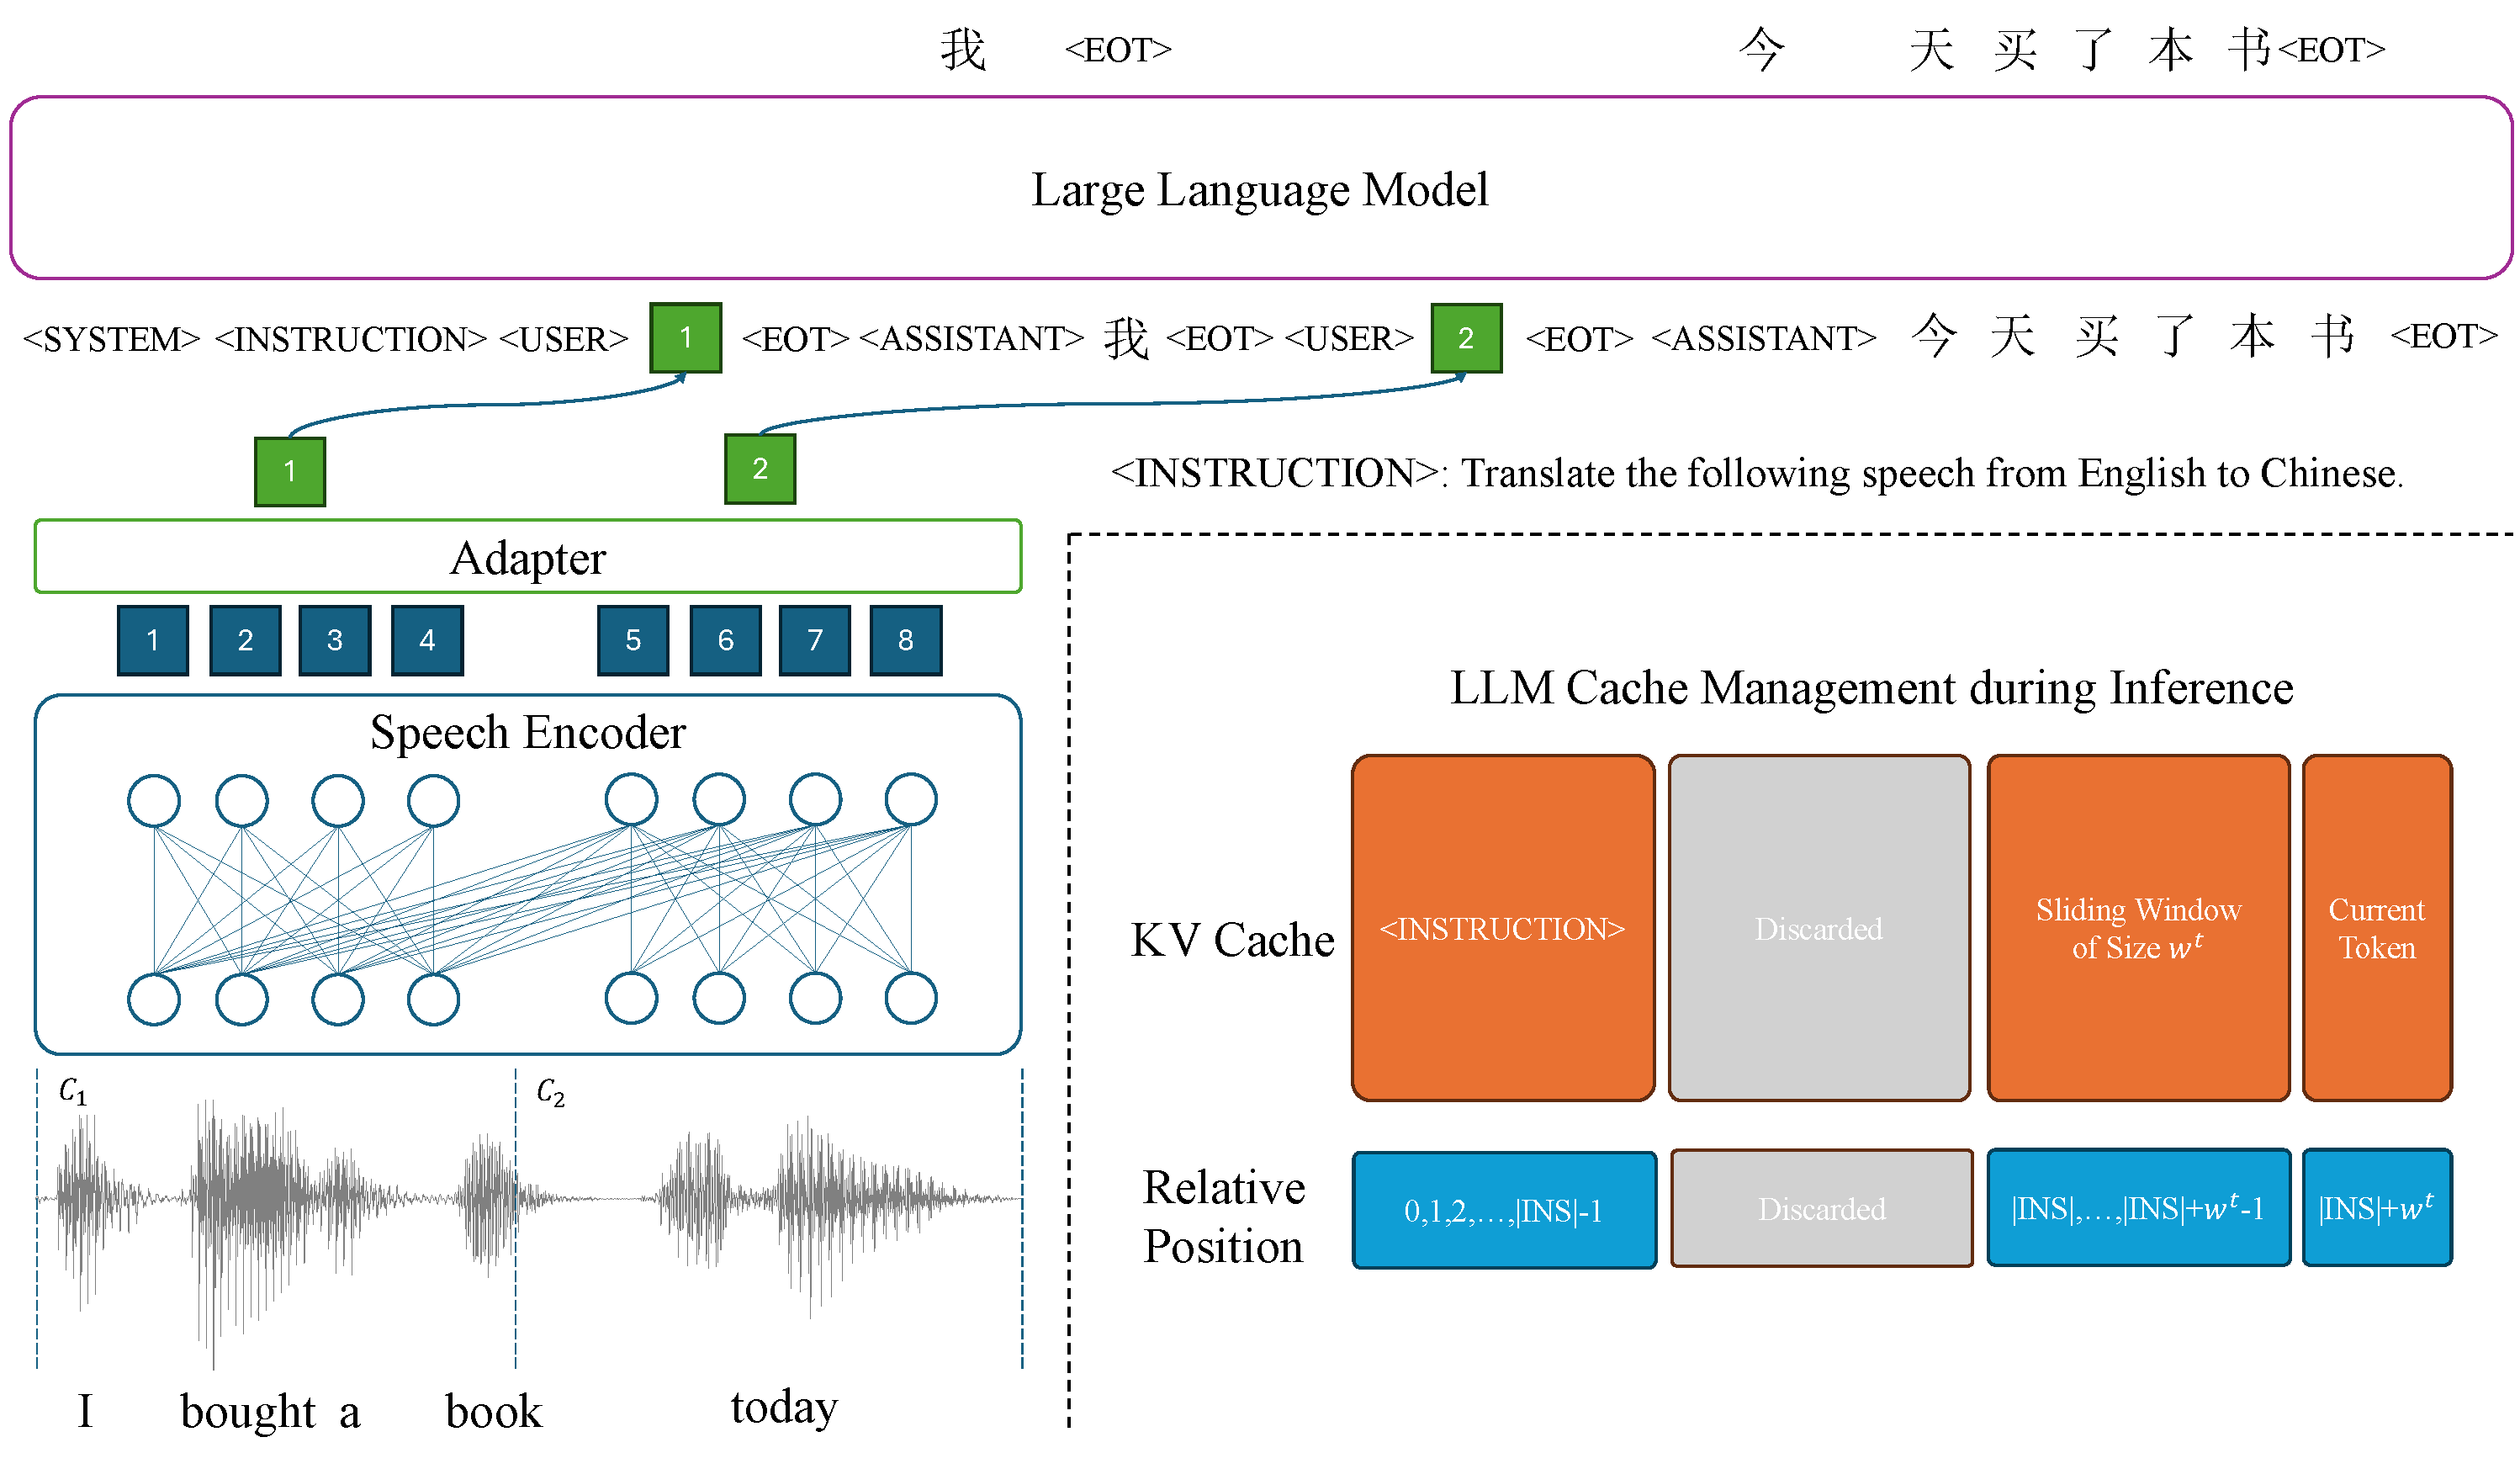
\includegraphics[width=0.9\linewidth]{fig/model.pdf}
    \caption{Overview of the proposed \method. }
    \label{fig:overview}
\end{figure}

\subsection{Overview}



The detailed framework of our method is shown in Figure~\ref{fig:overview}. To be specific, the end-to-end model accepts the original audio feature as input and outputs the target text 

\noindent\textbf{Problem Formulation}~xxxxxxx


\section{Experiments}
\label{sec:experiment}
List three research questions to verify in the experiments.
List claims for these question. 
List figures or tables needed as evidence to support the claims. 

\begin{figure}[htb]
    \centering
    ===Placeholder===
    \caption{Main result of XXXX. This figure shows that our proposed \method outperforms xxx by yyy points. }
    \label{fig:main_result}
\end{figure}



\begin{table}[htb]
    \centering
    ===Placeholder===
    \caption{Main result of XXX. This table shows our proposed \method outperforms xxxx by yyyy points. }
    \label{fig:main_result2}
\end{table}

\section{Analysis}
\label{sec:analysis}


TODO: Add your analysis section here. This could include error analysis, ablation studies, or detailed examination of your results.

\section{Conclusion}
\label{sec:conclusion}


TODO: Write your conclusion section here
We propose \method, a novel and unified training framework for jointly machine translation and text generation. 

\clearpage
\printbibliography

\newpage
\appendix
\section{Additional Details}
\label{sec:appendix}


TODO: Add any additional details, proofs, or supplementary material here.

\end{document}